\chapter{Classical {P}lanning}

\medskip\noindent
Before we dive into HTN planning, it's essential to understand its predecessor, which is classical planning or, as it is called in some literature, STRIPS planning~\cite{strips}. Classical planning is lightweight in the sense that it is easier to get into the theory of planning (independently on a representation of planning, which will be discussed in this chapter) and it is easier to describe domains of problems. The concept of classical planning is similar to the theory of Automata and Grammars (deterministic finite automaton (DFA), to be precise). There are different states of the world as well as actions that change one state to another. An action in classical planning can be viewed as a state transition function $\gamma: S \times A \rightarrow S$, where $S$ and $A$ denote the sets of all states and actions, respectively. If an action is applicable to a state then there will be a state transition, otherwise it will be undefined. The set of goal states, $S_g \subseteq S$, is analogous to a set of accepting states. The planning problem then can be reduced to a problem of searching paths in a directed graph.

\medskip\noindent
Although this approach to classical planning is simple and straightforward, it has one crucial flaw which makes it unusable in practice. Imagine a planning domain that describes a warehouse. If we have five locations, three piles of containers per location, three robots, and one hundred containers, then there are $10^{277}$ states~\cite{nau}, which is much more than the number of atoms in the observable universe. And that is just a simple small domain with a small amount of objects. For this purpose, we need to use better ways of representing classical planning, which will be called \emph{state-transition system}. We will briefly describe two possible representations: \emph{set-theoretic representation} and \emph{classical representation}.

\medskip\noindent
In both representations, the idea is to use more compact ways of defining a state of the world and actions that change the state. Instead of having a set of all states $S$, we will have a finite set of proposition symbols $P = \{p_1,\dots,p_n\}$ in \emph{set-theoretic representation} and a first-order language $\mathcal{L}$ in \emph{classical representation}. Both, $P$ and $\mathcal{L}$ describe properties and features of the world. Each state is then defined by a set of properties, which are true in that state and every other property is false. This feature is called closed world assumption. Both of these representations have the same expressive power~\cite{nau}. 

\medskip\noindent
All of the following definitions are correspondent and equivalent to the definitions in the book \emph{Automated Planning: theory and practice (Chapter 2)}~\cite{nau}.

\section{Set-Theoretic Representation}

\begin{defn}\label{def01:1}
  Let $P = \{p_1,\dots,p_n\}$ be a finite set of propositional symbols, which will model properties of a world. Then $\Sigma = (S, A, \gamma)$ is a \emph{planning domain} on $P$. $S$, $A$, and $\gamma$ denote the set of all states, set of all actions, and the \emph{state-transition function}, respectively, such that:

  \begin{itemize}
      \item $S \subseteq 2^{P}$, each state $s \in S$ is described by propositions that hold in that state. Other propositional symbols $p \in P$, $p \notin s$ do not hold in a state $s$.
      
      \item Each action $a \in A$ is defined as a triple of sets describing the preconditions and changes to a current state. Action $a \in A$ will be denoted as \mbox{$a=(pre(a), \text{eff}^{\,\,-}(a), \text{eff}^{\,\,+}(a)) \in  2^{P} \times 2^{P} \times 2^{P}$}, where $pre(a)$ stands for preconditions that must be true in a state to apply this action, meanwhile $\text{eff}^{\,\,-}(a)$ and $\text{eff}^{\,\,+}(a)$ describe changes to the state or, in other words, negative and positive effects\footnote{In some literature these sets are called: add list, delete list.}. We require $\text{eff}^{\,\,-}(a) \cap \text{eff}^{\,\,+}(a) = \emptyset$ for every $a \in A$, because otherwise it does not make any sense. Having a state $s \in S$, an action $a \in A$ is \emph{applicable} to state $s$, if and only if $pre(a) \subseteq s$ (it might be convenient to specify $pre^{-}(a)$ and $pre^{+}(a)$ to denote positive and negative preconditions).
      
      \item Having $s \in S$ and an action $a \in A$ that is \emph{applicable} to state $s$, \emph{state-transition} function $\gamma$ is defined as follows: $\gamma(s,a)=(s-\text{eff}^{\,\,-}(a)) \cup \text{eff}^{\,\,+}(a)$, otherwise it is undefined.
      \item $S$ must have a property that for every $s \in S$ and $a \in A$ that is \emph{applicable} to $s$, $\gamma(s,a) \in S$. This way we do not have to know all of the states in advance. All we need is a set of actions $A$ and some initial state $s_0 \in S$, then we can find all reachable states using Breadth-First Search (BFS), Depth-First Search (DFS), or some other searching algorithms.
  \end{itemize}
\end{defn}

\begin{defn}\label{def01:2}
  A \emph{planning problem} is a triple $\mathcal{P}=(\Sigma,s_o,g)$, such that:

  \begin{itemize}
    \item $\Sigma = (S, A, \gamma)$ is a \emph{planning domain} on $P$.
    
    \item $s_0 \in S$ is an \emph{initial state}.
    
    \item $g \subseteq P$ is a set of \emph{goal proposition symbol}, which must be true in the state after the final action of a plan. $S_g=\{s \in S | g \subseteq s\}$ is a set of goal states, i.e., states that satisfy the \emph{planning problem}~$\mathcal{P}.$
  \end{itemize}
\end{defn}

\noindent
Because the set of \emph{propositional symbol} $P$ is finite, sets of states, actions, and state-transition function are also finite.

\begin{defn}\label{def01:3}
  A \emph{plan} in a \emph{planning domain} $\Sigma$ is a finite sequence of actions $\pi=(a_1,\dots,a_k)$, where $k \geq 0$ and $(\forall a \in \pi) a \in A$. The \emph{plan} $\pi$ is \emph{applicable} to a state $s_0 \in S$, if and only if a sequence of states $(s_0,\dots,s_k)$ exist, such that: \mbox{$(1 \leq i \leq k)$} $pre(a_i) \subseteq s_{i-1}$ and $s_i = \gamma(s_{i-1},a_i) = ((s_{i-1}-\text{eff}^{\,\,-}(a_i)) \cup \text{eff}^{\,\,+}(a_i))$ is defined. Otherwise, the \emph{plan} $\pi$ is invalid. 

  \medskip\noindent
  In other words, a \emph{plan} $\pi=(a_1,\dots,a_k)$ is \emph{applicable} to a state $s_0$, if and only if a \emph{plan} $\pi'=(a_2,\dots,a_k)$ is \emph{applicable} to a state $s_1=\gamma(s_0,a_1) \in S$.

  \medskip\noindent
  Having a \emph{plan} $\pi=(a_1,\dots,a_k)$ and a state $s \in S$, we will abuse the notation to let $\gamma(s,\pi)$ denote a state $s_k \in S$, where we get after applying the sequence of actions of a plan, i.e.,
    \[
    \gamma(s,(a_1,\dots,a_k))=
    \begin{cases}
    s, & \text{if $k=0$ (there are no actions)},\\
    \gamma(\gamma(s,a_1),(a_2,\dots,a_k)), & \text{if k $>$ 0, $a_1$ is \emph{applicable} to $s$}, \\
    undefined, & \text{otherwise}.
    \end{cases}
    \]
\end{defn}



\begin{defn}\label{def01:4}
    A \emph{solution} to a \emph{planning problem} $\mathcal{P}=(\Sigma,s_o,g)$ is a plan $\pi=(a_1,\dots,a_k)$ that is \emph{applicable} to $s_0$, which changes the initial state $s_0$ to a state that satisfies \emph{goal propositional symbols}: $\gamma(s_0,\pi)$ is defined and $g \subseteq \gamma(s_0,\pi)$ (equivalent to $\gamma(s_0,\pi) \in S_g$).
\end{defn}

\noindent
For a \emph{planning problem} there might be many \emph{solutions}, moreover, there might be an infinite number of \emph{solutions} if there are states that can be visited repeatedly, (e.g. we might have two adjacent locations in a domain, that can be visited cyclically without any constraints).

\medbreak\noindent
It is easy to see that for each \emph{planning problem} $\mathcal{P}$ with nonempty set of \emph{solutions} (there exist a \emph{plan} $\pi$ such that $\pi$ is a solution to a $\mathcal{P}$) there exist at least one \emph{minimal solution} $\pi=(a_1,\dots,a_k)$, i.e., there is no \emph{solution} $\pi'=(a_1',\dots,a_j')$ such that $j < k$. There might be many different \emph{minimal solutions} but all of them share the same length.


\begin{example}\label{ex01:1}
    \begin{figure}
        \centering
        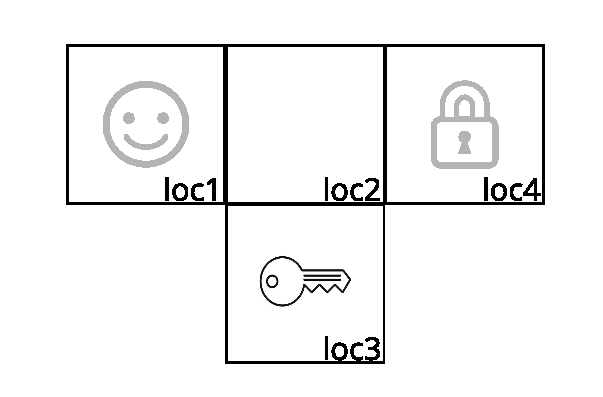
\includegraphics{img/output_mares_key1.pdf}
        \caption{Initial state of a simple planning domain}
        \label{fig01:1}
    \end{figure}
    
    Imagine a simple planning domain (Figure~\ref{fig01:1}) that can represent states in an uncomplicated maze-like game. We have four game locations, a player character, a key, and a locked door (illustrated by a \emph{loc4}). The character can move freely between locations but if he wants to enter \emph{loc4}, then he needs a key that can be picked at the \emph{loc3} (but cannot be discarded later on). Now we will define a planning problem $\mathcal{P}=(\Sigma,s_0,g)$ for this domain $\Sigma=(S,A,\gamma)$ more formally:
    
\end{example}

\begin{itemize}
    \item $P=\{${at-loc1,at-loc2,at-loc3,at-loc4,key-picked}$\}$,
    
    \item $S=\begin{aligned}[t]
    &\{\{ \mathrm{at\text{-}loc1}\}, \{ \mathrm{at\text{-}loc2}\}, \{ \mathrm{at\text{-}loc3}\}, \{ \mathrm{at\text{-}loc1,key\text{-}picked}\},\\
    & \{ \mathrm{at\text{-}loc2,key\text{-}picked}\},
    \{ \mathrm{at\text{-}loc3,key\text{-}picked}\}, \{ \mathrm{at\text{-}loc4,key\text{-}picked}\}\},
    \end{aligned}$

    \item $A=\begin{aligned}[t]
    &\mathrm{\{move12,move21,move23,move32,move24,move42,pick\}, where:} \\
    &\mathrm{move12 = (\{at\text{-}loc1\},\{at\text{-}loc1\},\{at\text{-}loc2\});} \\
    &\mathrm{move21 = (\{at\text{-}loc2\},\{at\text{-}loc2\},\{at\text{-}loc1\});} \\
    &\mathrm{move23 = (\{at\text{-}loc2\},\{at\text{-}loc2\},\{at\text{-}loc3\});} \\
    &\mathrm{move32 = (\{at\text{-}loc3\},\{at\text{-}loc3\},\{at\text{-}loc2\});} \\
    &\mathrm{move24 = (\{at\text{-}loc2,key\text{-}picked\},\{at\text{-}loc2\},\{at\text{-}loc4\});} \\
    &\mathrm{move42 = (\{at\text{-}loc4\},\{at\text{-}loc4\},\{at\text{-}loc2\});} \\
    &\mathrm{pick = (\{at\text{-}loc3\},\{\},\{key\text{-}picked\}),}
    \end{aligned}$ 

    \item $\gamma$ as defined in Definition~\ref{def01:1},

    \item $s_0 = \{ \mathrm{at\text{-}loc1}\}$ (Figure~\ref{fig01:1}),

    \item $g = \{ \mathrm{at\text{-}loc4, key\text{-}picked}\}$.
\end{itemize}

\noindent
Example~\ref{ex01:1} shows us a complete description of a \emph{planning domain} $\Sigma$ and a \emph{planning problem} $\mathcal{P}$. There is one and only \emph{minimal solution} which is $\pi=(\mathrm{move12,move23,pick,move32,move24})$. On the other hand, there is an infinite number of \emph{solutions}. We might go to the loc3 and apply the action pick as many times as we desire, thus generating an infinite amount of \emph{solutions}.

\medskip\noindent
With knowledge of the particular domain, we can adjust the domain without losing any domain's specifics. For example, we might alter the set of the \emph{goal proposition symbols} $g$ to be $g=\mathrm{\{at\text{-}loc4\}}$ because we know that it is impossible to enter loc4 without having a key picked up at the loc3.

\medskip\noindent
The set of states $S$ contains all reachable states from the initial state $s_0$, other unreachable states might be added to the $S$ but they are not needed. For example, the state \{at-loc1,at-loc2\} is contradictory because we cannot be at two locations simultaneously. Likewise states \{\}, \{key-picked\}, \{at-loc4\} are also meaningless.

\medskip\noindent
The concept of the key in this domain is depicted as \emph{a propositional symbol} key-picked. This simplification does not take into account the location of a key because it is not needed in this domain. Once the key is picked, it will be implicitly located at the same location as the character. Hence, the action pick is \emph{applicable} more than once in a \emph{plan}.

\begin{figure}
    \centering
    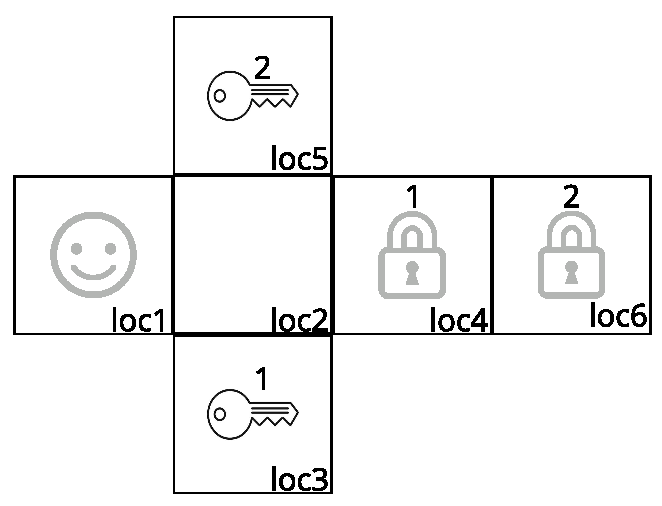
\includegraphics{img/output_mares_key2.pdf}
    \caption{Extended planning domain of a maze-like game}
    \label{fig01:2}
\end{figure}

\begin{example}\label{ex01:2}
    Let's consider an extension of this domain by adding two new locations, and another key (Figure~\ref{fig01:2}). Only this time we want to model a new constraint that allows at most one key to be held at a time. There are numerous ways of modeling this planning domain. For instance, we might introduce new \emph{propositional symbols}: \emph{key1-picked, key2-picked, door1-opened, door2-opened}. If we wanted to model the locations of keys, we would need to include many new \emph{propositional symbols} of the form \emph{key1-at-loc1, key1-at-loc2}, and so on. Also, we would need new \emph{actions} that would consider the locations of a key and the character. New actions may look like this: \emph{pick-key1-at1 = (\{at-loc1,key1-at-loc1\},\{key2-picked\},\{key1-picked\}), move12-with-key1 = (\{at-loc1,key1-at-loc1\},\{at-loc1,key1-at-loc1\},\{at-loc2,key1-at-loc2\})} and so on. This enumeration of possible substates might result in an enormous set of \emph{propositional symbols} and other related sets \emph{\cite{nau}~{(2.2.4 Properties of the Set-Theoretic Representation)}}. An elaborate solution that fixes this problem is discussed in the following chapter.
\end{example}

\section{Classical Representation}\label{class_repre}

\noindent
\emph{Classical representation} of planning improves \emph{set-theoretic representation} by introducing a first-order language $\mathcal{L}$ that consists of a finite number of constant symbols (similar to a set of \emph{propositional symbols} defined in Definition~\ref{def01:1}), predicate symbols, and other symbols for the representation of \emph{planning operators}. We do not allow any functional symbols in $\mathcal{L}$ because we are focused to model finite models where functions are not needed. A state in \emph{classical representation} is defined as a set of grounded logical atoms of $\mathcal{L}$.

\begin{example}\label{ex01:3}
    Before we start with definitions, we will look at Figure~\ref{fig01:1} from the perspective of \emph{classical planning}. We want to model the player, key, locations, and locked door. Thus, the set of constant symbols is \emph{\{player,loc1,loc2,loc3,loc4} \emph{,key1,nothing,door\}}. The constant symbol \emph{nothing} represents that the player's inventory is empty. With this knowledge, we can represent the initial state of Figure~\ref{fig01:1} to be $s_0=\{\mathrm{adjacent(loc1,loc2)},\mathrm{adjacent(loc2,loc1)},\mathrm{adjacent(loc2,loc3)}, \\ \mathrm{adjacent(loc3,loc2)}, \mathrm{adjacent(loc2,loc4)},\mathrm{adjacent(loc4,loc2)}, \mathrm{at(player,loc1)}, \\ \mathrm{holds(player,nothing)}, \mathrm{locked(door)}\}$. Some logical atoms will remain the same throughout all possible states, e.g. \emph{adjacent(loc1,loc2)}, meanwhile other atoms like \emph{at(player,loc1)} or \emph{holds(player,nothing)} will change after the application of proper actions.
\end{example}

\medskip\noindent
Now we will define \emph{planning operators} in \emph{classical planning}. A grounded instance of an operator is an action that can be part of a \emph{plan}.

\pagebreak

\begin{defn}\label{def01:5}
    A \emph{planning operator} is a triple $o = (name(o),precond(o), \\ \text{eff}(o))$, where:

        \begin{itemize}
            \item $name(o)$ is of a form $n(x_1,\dots,x_k)$, where $n$ is a \emph{operator symbol} and must be unique in $\mathcal{L}$ and $x_1,\dots,x_k$ represent variable symbols that appear in an operator,

            \item $precond(o)$ and $\text{eff}(o)$ generalize preconditions and effects of \emph{set-theoretic representation}. These sets contain positive and negative logical literals.
        \end{itemize}

    Let $O$ denote a set of all \emph{planning operators} as specified above.
\end{defn}

\medskip\noindent
In some literature, the usage of $name(o)$ is not specified, rather the multiset of grounded operators (actions) is assumed. The essence of $name(o)$ is in the planning phase. We might have multiple grounded instances of operators that might use the equivalent constant symbols. To help differentiate a \emph{planning operator} from an instance of a \emph{planning operator}, the $name(o)$ might come in handy. $name(o)$ refers unambiguously to one specific \emph{planning operator}. We will omit the usage $name(o)$ because the meaning will be obvious from the context.


\begin{example}\label{ex01:4}
    In this example, we will look at some possible \emph{planning operators} that might be used in Figure~\ref{fig01:2} (we will use new predicate symbols that were not specified yet):

    \begin{itemize}
        \item \emph{move(player,location1,location2)} \\
        precond: \emph{adjacent(location1,location2), at(player,location1), \neg locked(location2)} \\
        effects: \emph{\neg at(player,location1), at(player, location2)}

        \item \emph{pickup-key(player,key,location)} \\
        precond: \emph{at(player,location), at(key,location), holds(player,nothing)} \\
        effects: \emph{\neg holds(player,nothing), \neg at(key,location), holds(player,key)}

        \item \emph{drop-key(player,key,location)} \\
        precond: \emph{at(player,location), holds(player,key)} \\
        effects: \emph{\neg holds(player,key), at(key,location), holds(player,nothing)}

        \item \emph{open-door(player,location1,location2, key)} \\
        precond: \emph{adjacent(location1,location2), locked(location2), at(player,location1), key-opens-door(key,location2), holds(player,key)} \\
        effects: \emph{\neg locked(location2)}
    \end{itemize}
\end{example}

\medskip\noindent
In the Example~\ref{ex01:4} predicate symbols adjacent(l1,l2) and key-opens-door(key,location) are describing static properties of a domain that will never change and thus, will never appear in effects of \emph{planning operators}. On the other hand, predicate symbols like at(player/key,location), locked(location), or holds(player, key) will change and therefore will occur in effects of \emph{planning operators}.

\begin{defn}\label{def01:6}
Let us be given a state $s \in S$ and an action (ground instance of a \emph{planning operator}) $a$. If $precond^{+}(a) \subseteq s$ and $precond^{-}(a) \cap s = \emptyset$, where $precond^{+}(a)$ denotes a set of all positive atoms in $precond(a)$ and $precond^{-}(a)$ denotes a set of all atoms whose negation is in $precond(a)$, then $a$ is \emph{applicable} to $s$ and $\gamma(s,a)=(s-\text{eff}^{\,\,-}(a)) \cup \text{eff}^{\,\,+}(a)$. $\text{eff}^{\,\,-}(a)$ and $\text{eff}^{\,\,+}(a)$ are analogous to $precond^{-}(a)$ and $precond^{+}(a)$, respectively.
\end{defn}

\begin{defn}\label{def01:7}
Having a first-order language $\mathcal{L}$ with a finite amount of constant and predicate symbols and no functional symbols, the \emph{classical planning domain} in $\mathcal{L}$ is a state-transition system $\Sigma = (S,A,\gamma)$ such that:

    \begin{itemize}
        \item $S \subseteq 2^{\displaystyle \{all~ground~atoms~of~\mathcal{L}\}}$,
        
        \item $A =~$\{all ground instances of operators in $O$\},
        
        \item $\gamma$ is analogous Definition~\ref{def01:1},
        
        \item $S$ is closed under $\gamma$ in the same manner as in Definition~\ref{def01:1}.
    \end{itemize}
\end{defn}

\begin{defn}\label{def01:8}
A \emph{classical planning problem} is corresponding to \emph{set-theoretic planning problem}, it is defined as $\mathcal{P} = (\Sigma,s_0,g)$, where:

    \begin{itemize}
        \item $\Sigma = (S,A,\gamma)$ is a \emph{classical planning domain},
        
        \item $s_0 \in S$ is an initial state
        
        \item $g$ is a set of literals.
    \end{itemize}
\end{defn}
